\documentclass{bmvc2k}

%% Enter your paper number here for the review copy
%\bmvcreviewcopy{??}

%\usepackage[brazilian]{babel}
\usepackage[utf8]{inputenc}
\usepackage{bm}
\usepackage{amsmath}
\usepackage{tabularx}
\usepackage{siunitx}

\title{Projeto Demonstrativo 3}

% Enter the paper's authors in order
% \addauthor{Name}{email/homepage}{INSTITUTION_CODE}
\addauthor{Pedro Henrique Luz de Araujo}{pedrohluzaraujo@gmail.com}{1}
\addauthor{Rafael Barbosa de Sousa}{rafael.1940.b@gmail.com}{1}

% Enter the institutions
% \addinstitution{Name\\Address}
\addinstitution{
  Departamento de Ci\^encia da Comptuta\c{c}\~ao\\
  Universidade de Bras\'{\i}lia\\
  Campus Darcy Ribeiro, Asa Norte\\
  Bras\'{\i}lia-DF, CEP 70910-900, Brazil,  
}

\runninghead{Luz de Araujo, P.H.; de Sousa, R. B.}{PD3 -- \today}

% Any macro definitions you would like to include
% These are not defined in the style file, because they don't begin
% with \bmva, so they might conflict with the user's own macros.
% The \bmvaOneDot macro adds a full stop unless there is one in the
% text already.
\def\eg{\emph{e.g}\bmvaOneDot}
\def\ie{\emph{i.e}\bmvaOneDot}
\def\Eg{\emph{E.g}\bmvaOneDot}
\def\etal{\emph{et al}\bmvaOneDot}
\newcommand{\norm}[1]{\left\lVert#1\right\rVert}
\newcommand\blfootnote[1]{%
  \begingroup
  \renewcommand\thefootnote{}\footnote{#1}%
  \addtocounter{footnote}{-1}%
  \endgroup
}


%-------------------------------------------------------------------------
% Document starts here
\begin{document}
\begin{NoHyper}
\maketitle
\end{NoHyper}

\begin{abstract}
O presente Projeto Demonstrativo visa a implementar um programa capaz de estimar a profundidade de uma cena dadas imagens obtidas por duas câmeras. Para tanto, calcula-se um mapa de disparidade da cena por meio da minimização da soma das diferenças absolutas (SAD) dos pixeis correspondentes nas duas imagens em caso de câmeras paralelas. No caso de câmeras não paralelas, as imagens são retificadas e então é minimizada a SAD. A partir da visão estéreo, obtivemos uma matriz de transformação dos pontos da imagem para o mundo, de modo que foi possível calcular dimensões reais a partir de imagens.\footnote{Pedro contribuiu com a elaboração do código principal do projeto e com a escrita da introdução, metodologia e resultados. Rafael contribuiu com estruturação do código e do relatório e com a escrita da introdução e metodologia.}
\end{abstract}

%-------------------------------------------------------------------------
\section{Introdução}
\label{sec:intro}

Um dos ramos da Visão Computacional é a visão estéreo, que se ocupa da reconstrução espacial da cena a partir de duas visões diferentes~\cite{Hartley:2003:MVG:861369}. Isto é, dado um conjunto de correspondência em imagens $\bm{x_i} \leftrightarrow \bm{x'_i}$, obtidos de um conjunto de pontos tridimensionais desconhecidos $\bm{X_i}$, a recuperação espacial da cena visa a achar as matrizes $\mathbf{P}$ e $\mathbf{P'}$ tais que
\begin{equation}
\centering
\label{Pmatrix}
\bm{x_i}=\mathbf{P}\bm{X_i}~\text{e}~ \bm{x'_i}=\mathbf{P'}\bm{X_i}~\text{para todo}~i\,.
\end{equation}

No caso de visões obtidas de câmeras idênticas e perfeitamente paralelas (figura~\ref{paralel}), basta saber a distância entre os centros das câmeras, denominada \textit{baseline} ($b$), e a distância focal das câmeras ($f$), como evidenciam as equações abaixo:

\begin{figure}[htb] 
\centering
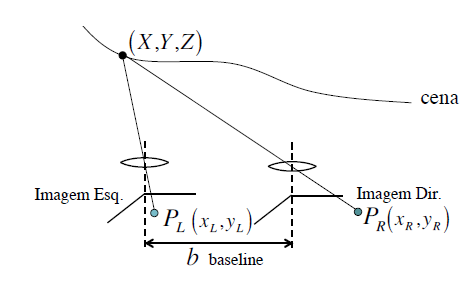
\includegraphics[width=0.5\textwidth]{figs/stereo.png}
\caption{Disparidade e profundidade em câmeras paralelas. Imagem adaptada dos slides de D. A. Forsyth.\label{paralel}}
\end{figure}

\begin{equation}
    \label{eq_disp}
    X = \frac{b(x_l + x_r)}{2(x_l - x_r)},
    Y = \frac{b(y_l + y_r)}{2(x_l - x_r)},
    Z = \frac{bf}{(x_l - x_r)}\,.
\end{equation}

A medida $x_l - x_r$ é denominada disparidade e indica a diferença entre a localização de um mesmo ponto nas duas imagens e é inversamente proporcional à profundidade do ponto. Logo, para estimar a profundidade dos pontos da cena é preciso calcular a disparidade de todos os pontos. 

No caso em questão, de câmeras paralelas, as coordenadas dos pontos correspondentes possuem o mesmo valor no eixo $y$. Assim, para encontrar a correspondência de um ponto na outra imagem basta procurar o pixel mais semelhante na mesma fileira do ponto original. Uma medida de semelhança comumente usada é a diferença absoluta, que corresponde à norma $l_1$ da diferença entre o valor dos pixeis. Por exemplo, no caso de um pixel com três canais:

\begin{equation}
    \label{norma}
    AD = |\bm{p} - \bm{p'}|_1 = |x - x'| + |y - y'| + |z - z'|\,.
\end{equation}

Por outro lado, busca pixel a pixel pode acarretar numa disparidade muito ``barulhenta'' (\textit{noisy}) ou irregular. Para suavizar (\textit{smooth}) a disparidade, pode-se encontrar correspondência entre janelas de pixeis - quanto maior a janela, maior a suavização da disparidade. Nesse caso, busca-se minimizar a soma das diferenças absolutas (SAD):
\begin{equation}
    \label{SAD}
    SAD = \sum_i |\bm{p_i} - \bm{p'_i}|\,.
\end{equation}

Em caso de visões obtidas de câmeras não paralelas, os pontos correspondentes não possuem necessariamente o mesmo valor em $y$. Torna-se necessário, portanto, diminuir o número de possibilidades dentre os pixeis que podem ser selecionados como correspondentes. Se soubermos os parâmetros extrínsecos e intrínsecos de cada câmera, podemos utilizar as matrizes de rotação e translação de cada uma delas para retificar as imagens, isto é, fazer os pixeis correspondentes terem uma das coordenadas iguais, como demonstram as imagens~\ref{before} e~\ref{after}.

Uma vez retificadas as imagens, basta aplicar o mesmo algoritmo usado para o caso de câmeras paralelas.

\begin{figure}[htb]
\centering
\begin{minipage}[t]{0.45\textwidth}
  \centering
  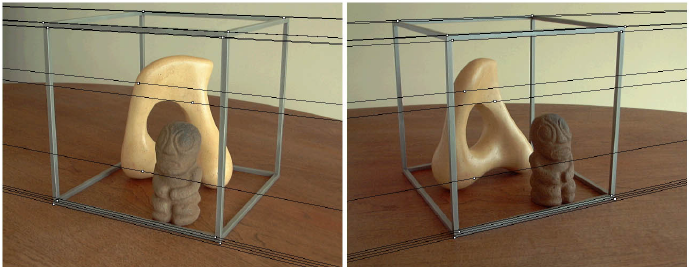
\includegraphics[width=\linewidth]{figs/homografphy1.png}
  \caption{Imagens antes da retificação.}
  \label{before}
\end{minipage}\hfill
\begin{minipage}[t]{0.45\textwidth}
  \centering
  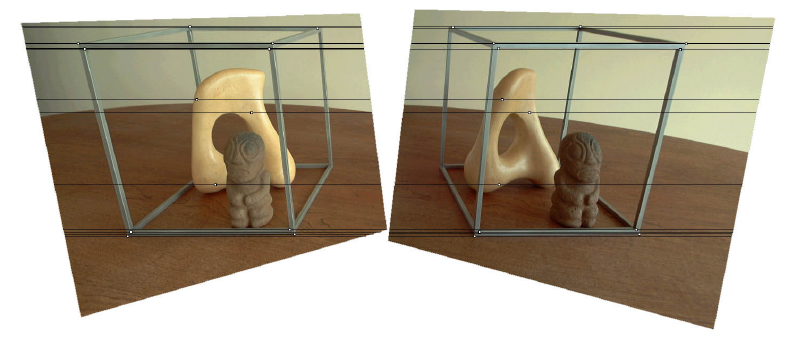
\includegraphics[width=\linewidth]{figs/homography2.png}
  \caption{Imagens após retificação.}
  \label{after}
\end{minipage}
\end{figure}


\section{Metodologia}
\label{sec:met}

\subsection{Ferramentas}
Usamos a biblioteca OpenCV~\cite{opencv_library}, versão 3.3.0, com implementações eficientes de algoritmos de correspondência estéreo e de reprojeções de imagens. Para realizar operações sobre matrizes e vetores, utilizamos a biblioteca de computação numérica em Python, NumPy. Usamos ainda, como linguagem, Python 3.5.2, e o gerenciador de bibliotecas Anaconda 3.

\subsection{Requisito 1}
O objetivo do requisito 1 é obter os mapas de disparidade e profundidade de imagens obtidas de câmeras paralelas, de modo que os pontos correspondentes nas duas imagens possuem o mesmo valor da coordenada $y$.

Dadas duas imagens pelo usuário, da esquerda e da direita, empregamos a classe \textit{StereoBM} da biblioteca OpenCV para obter a disparidade para cada ponto das imagens. De posse da matriz de disparidades, é possível obter as coordenadas do ponto na cena espacial por meio das equações \ref{eq_disp}. A distância focal das câmeras e o baseline são dados e valem 3640 pixeis e 160 mm, respectivamente. O tamanho da janela e o número máximo de disparidade para a minimização da SAD podem ser escolhidos livremente pelo usuário por meio de interface gráfica, como mostra a imagem~\ref{fig:trackbar}.

\begin{figure}[htb] 
\centering
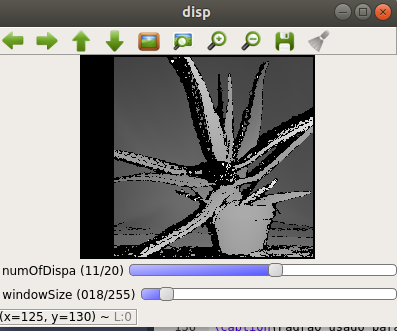
\includegraphics[width=0.3\textwidth]{figs/trackbar.png}
\caption{Interface gráfica de ajuste de parâmetros. Máximo de disparidade ajustado em 176 ($16 \times 11$, vez que o OpenCV só permite múltiplos de 16 na disparidade) e tamanho da janela ajustado em 19 ($18 + 1$, pois o OpenCV só permite janelas de tamanho ímpar). \label{fig:trackbar}}
\end{figure}

A partir dos valores de disparidade e de profundidade obtidos, normalizamos os valores e construímos uma imagem para o mapa de disparidade e outra para o mapa de profundidade. A normalização foi feita da seguinte forma:

Para o mapa de disparidade, ajustamos os valores de forma que a maior disparidade seja 255 e a menor seja 0. Como a disparidade é inversamente proporcional à profundidade, isso significa que quanto mais próximo o ponto mais claro ele será; quanto mais distante, mais escuro.

Para o mapa de profundidade, a normalização é semelhante. Os valores são ajustados de modo que profundidades infinitas ou onde não foi possível calculá-la possuam o valor 255 e a menor profundidade seja 0. Dessa forma, o mapa de profundidade é quase um negativo do mapa de disparidade: quanto mais próximo o ponto, mais perto de preto ele será; quanto mais distante, mais perto de branco.

\subsection{Requisito 2}
O requisito 2, assim como o requisito 1, tem como objetivo a construção de mapa de disparidade e profundidade para uma cena. Entretanto, as câmeras não mais são paralelas, de modo que torna-se necessário retificar as imagens.

Sabendo os parâmetros intrínsecos e extrínsecos de cada câmera, procedemos a retificação das imagens da seguinte maneira. Sejam 
$\mathbf{A_1}$, $\mathbf{A_2}$, $\mathbf{R_1}$, $\mathbf{R_2}$, $\bm{t_1}$ e $\bm{t_2}$ as matrizes de intrínsecos e de rotação e os vetores de translação da primeira e segunda câmera, respectivamente. Podemos obter a matriz de rotação $\mathbf{R}$ e o vetor de translação $\bm{t}$ entre a primeira e a segunda câmera da seguinte maneira:

\begin{subequations}
    \begin{align}
    \mathbf{R}&=\mathbf{R_2}\mathbf{R_1^t}\\
    \bm{t}&=\bm{t_2}-\mathbf{R}\bm{t_1}\,.
    \end{align}
\end{subequations}

De posse da rotação e da translação entre as câmeras, podemos rotacionar e transladar as imagens de forma que os planos das imagens se tornem paralelas e os pontos correspondentes possuam o mesmo valor da coordenada $y$. As funções \textit{stereoRectify}, \textit{initUndistortMap} e \textit{remap}, do OpenCV, fazem exatamente isso. A função \textit{stereoRectify} nos retorna, ainda, uma matriz $\mathbf{Q}$ que transforma disparidade em profundidade~\cite{Bradski:2013:LOC:2523356},
\begin{equation}
    \centering
    \mathbf{Q} = \begin{bmatrix}
    1 & 0 & 0 & -c_x  \\
    0 & 1 & 0 & -c_y  \\
    0 & 0 & 0 & f \\
    0 & 0 & \frac{-1}{T_x} & \frac{c_x - c'_x}{T_x}
    \end{bmatrix}\,,
\end{equation}
em que $c_x$ e $c_y$ são as coordenadas do ponto principal da primeira câmera, $c'_x$ é a coordenada x do ponto principal da segunda câmera, $f$ é a distância focal e $T_x$ é a \textit{baseline}.

Após retificarmos as imagens, aplicamos a mesma técnica do requisito 1 para obter os mapas de disparidade e profundidade da cena. Entretanto, em vez de usar as equações~\ref{eq_disp} para encontrar a profundidade, usamos a matriz $\mathbf{Q}$:
\begin{subequations}
    \begin{align}
    \begin{bmatrix}
    X \\
    Y  \\
    Z \\
    W
    \end{bmatrix}
    &=
    \mathbf{Q}\begin{bmatrix}
    x \\
    y  \\
    d\\
    1
    \end{bmatrix}\\
    \bm{p} &= \begin{bmatrix}
    \frac{X}{W} \\
    \frac{Y}{W}  \\
    \frac{Z}{W} 
    \end{bmatrix}\,,
    \end{align}
\end{subequations}
em que $d$ é a disparidade do ponto e $\bm{p}$ são as suas coordenadas no espaço.

\subsection{Requisito 3}
\label{met3}
Para o requisito 3 deseja-se obter as dimensões da menor caixa capaz de guardar a poltrona onde está posicionado o boneco Morpheus (figuras~\ref{fig:morpheusL} e~\ref{fig:morpheusR}).

O requisito 2 já fornece uma técnica capaz de obter as coordenadas no mundo real a partir dos pontos na imagem. Portanto, para o requisito 3, desenvolvemos uma aplicação em que o usuário clica em dois pontos e o sistema fornece a distância (norma da diferença entre os pontos) entre os dois pontos em milímetros no mundo real. Assim, medimos três vetores: de largura, de altura e de profundidade. Medimos cada uma dessas distâncias três vezes e calculamos a média e o desvio padrão entre elas, descartando \textit{outliers} evidentes.

\begin{figure}[htb]
\centering
\begin{minipage}[t]{0.35\textwidth}
  \centering
  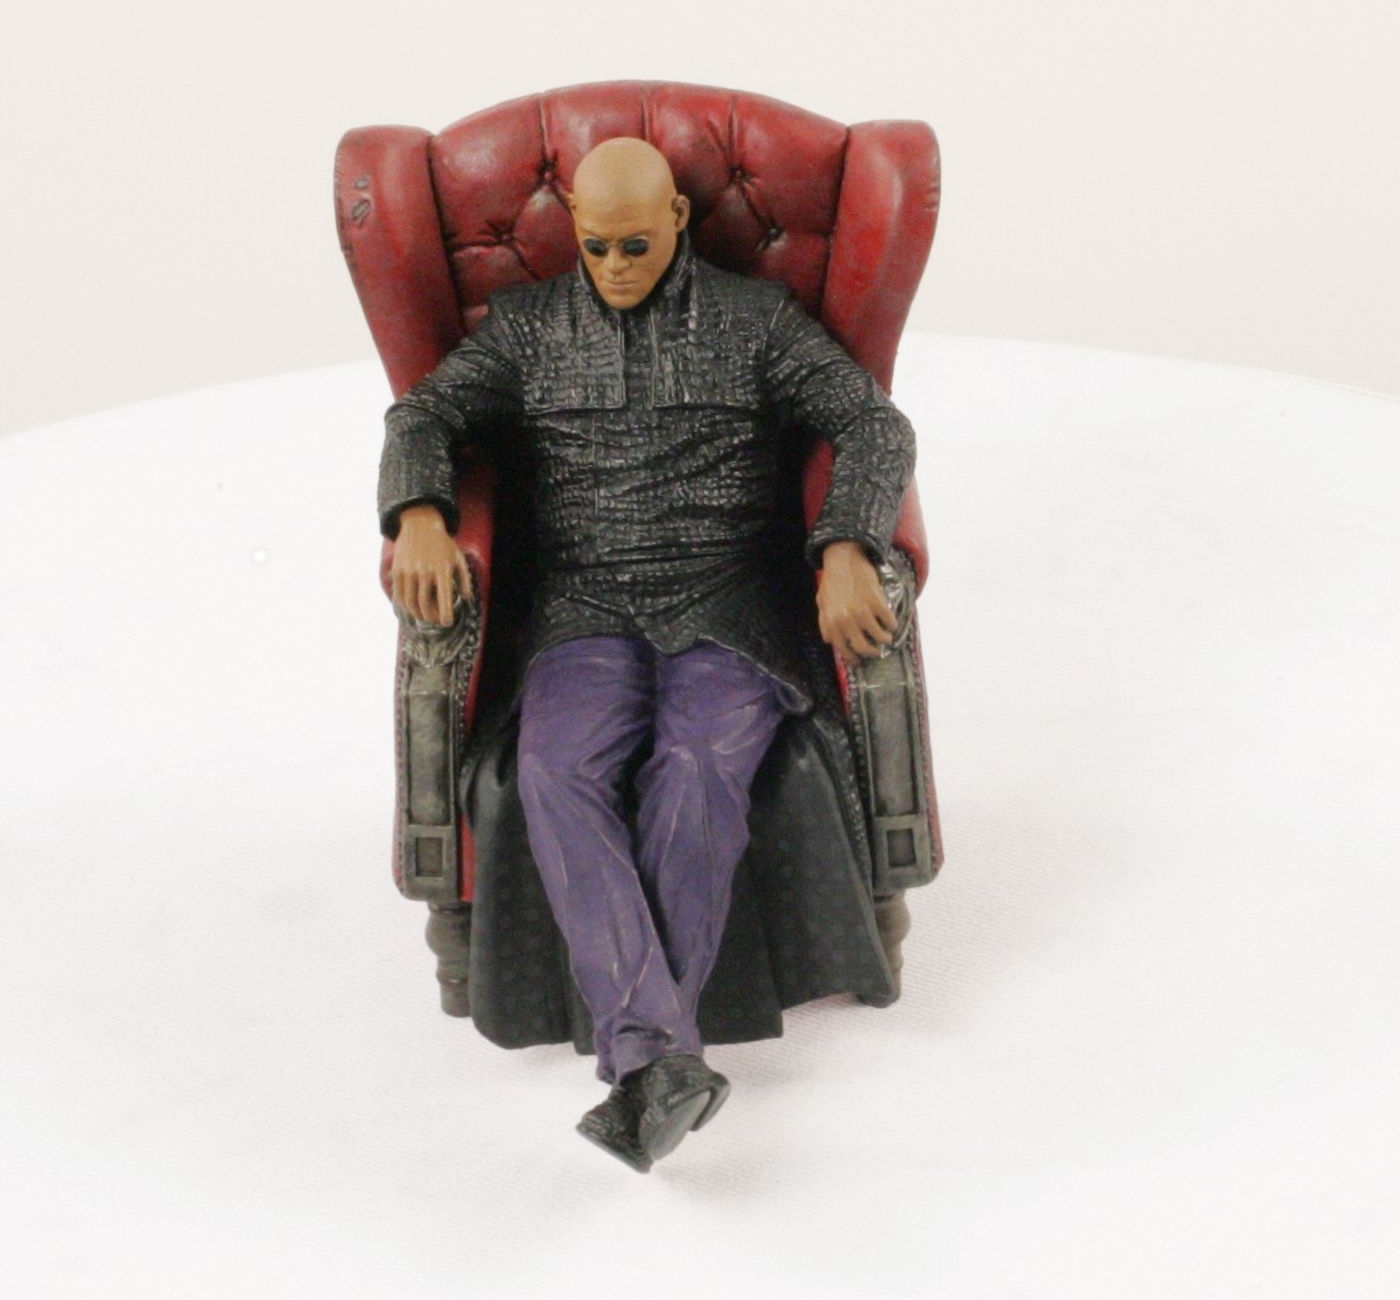
\includegraphics[width=\linewidth]{figs/MorpheusL.jpg}
  \caption{Imagem capturada pela câmera 1.}
  \label{fig:morpheusL}
\end{minipage}
\begin{minipage}[t]{0.35\textwidth}
  \centering
  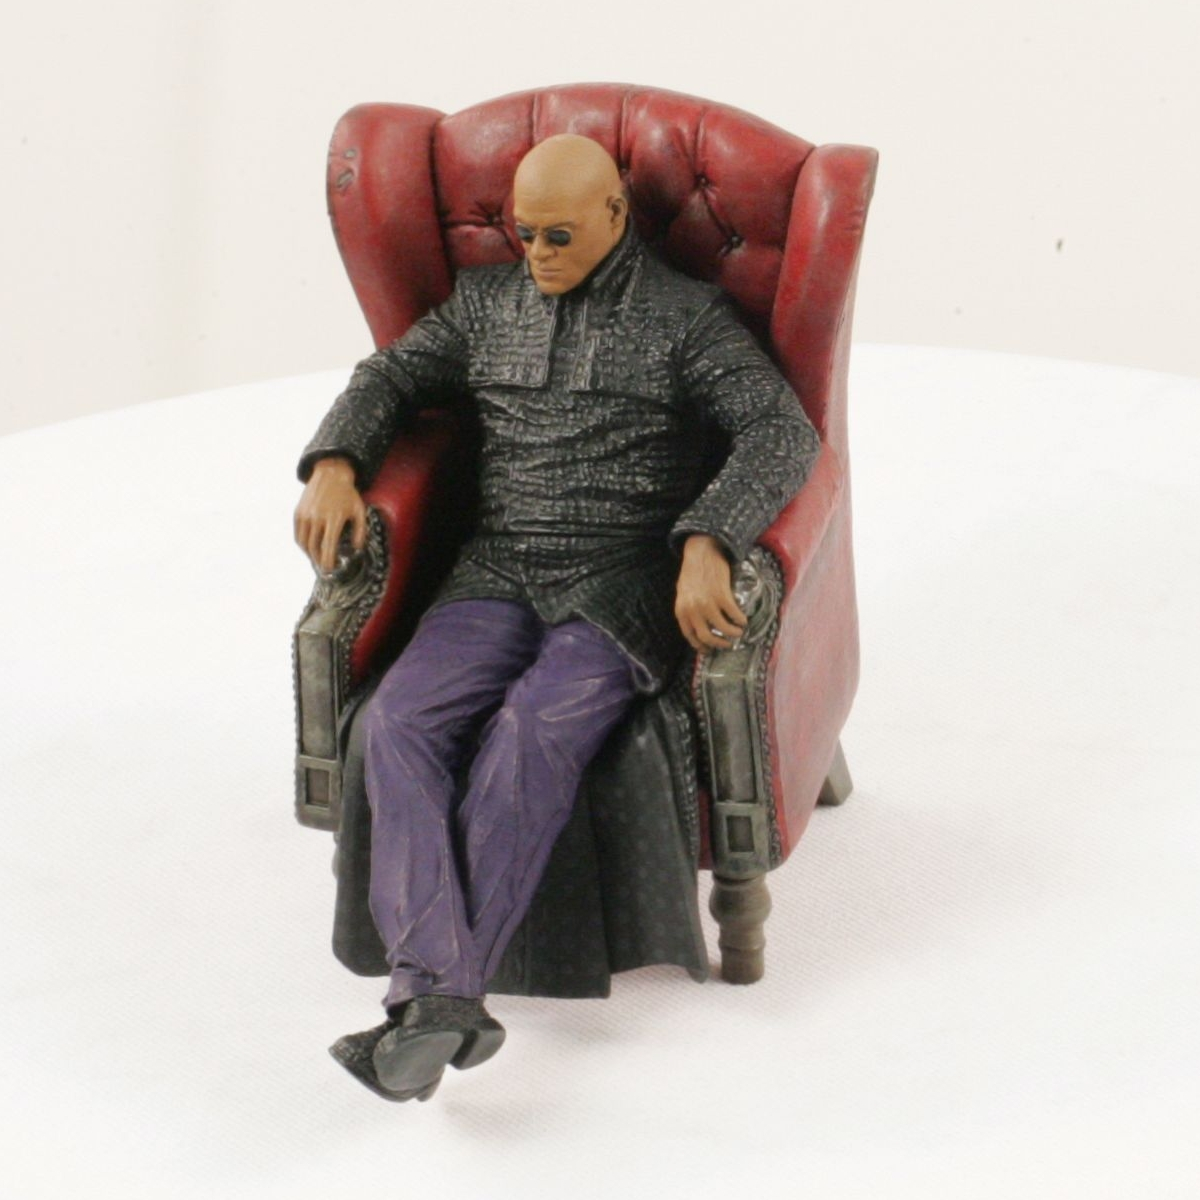
\includegraphics[width=\linewidth]{figs/MorpheusR.jpg}
  \caption{Imagem capturada pela câmera 2.}
  \label{fig:morpheusR}
\end{minipage}
\end{figure}

\section{Resultados}
\label{sec:res}
\subsection{Requisito 1}
As figuras~\ref{fig:aloeL} e~\ref{fig:aloeR} são as duas capturas da imagem de uma planta. As figuras~\ref{fig:aloe_disp} e~\ref{fig:aloe_depth} são, respectivamente, o mapa de disparidade e profundidade da cena, obtidos com uma janela de tamanho 15 e um número máximo de disparidade igual a 176.

\begin{figure}[htb]
\centering
\begin{minipage}[t]{0.2\textwidth}
  \centering
  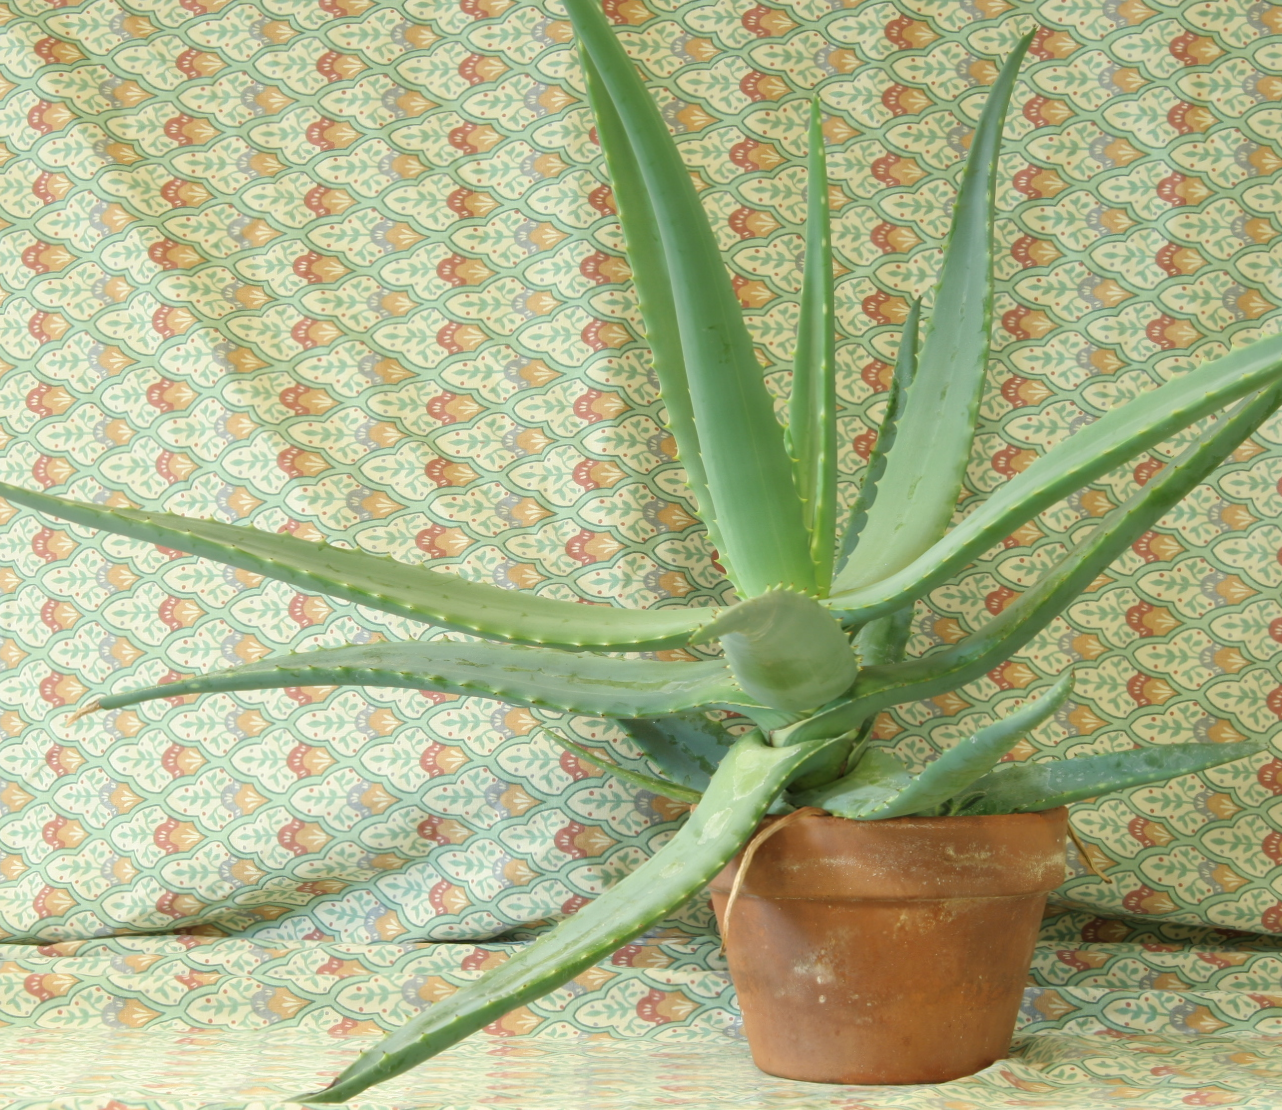
\includegraphics[width=\linewidth]{figs/aloeL.png}
  \caption{Planta pela câmera da esquerda.}
  \label{fig:aloeL}
\end{minipage}\hfill
\begin{minipage}[t]{0.2\textwidth}
  \centering
  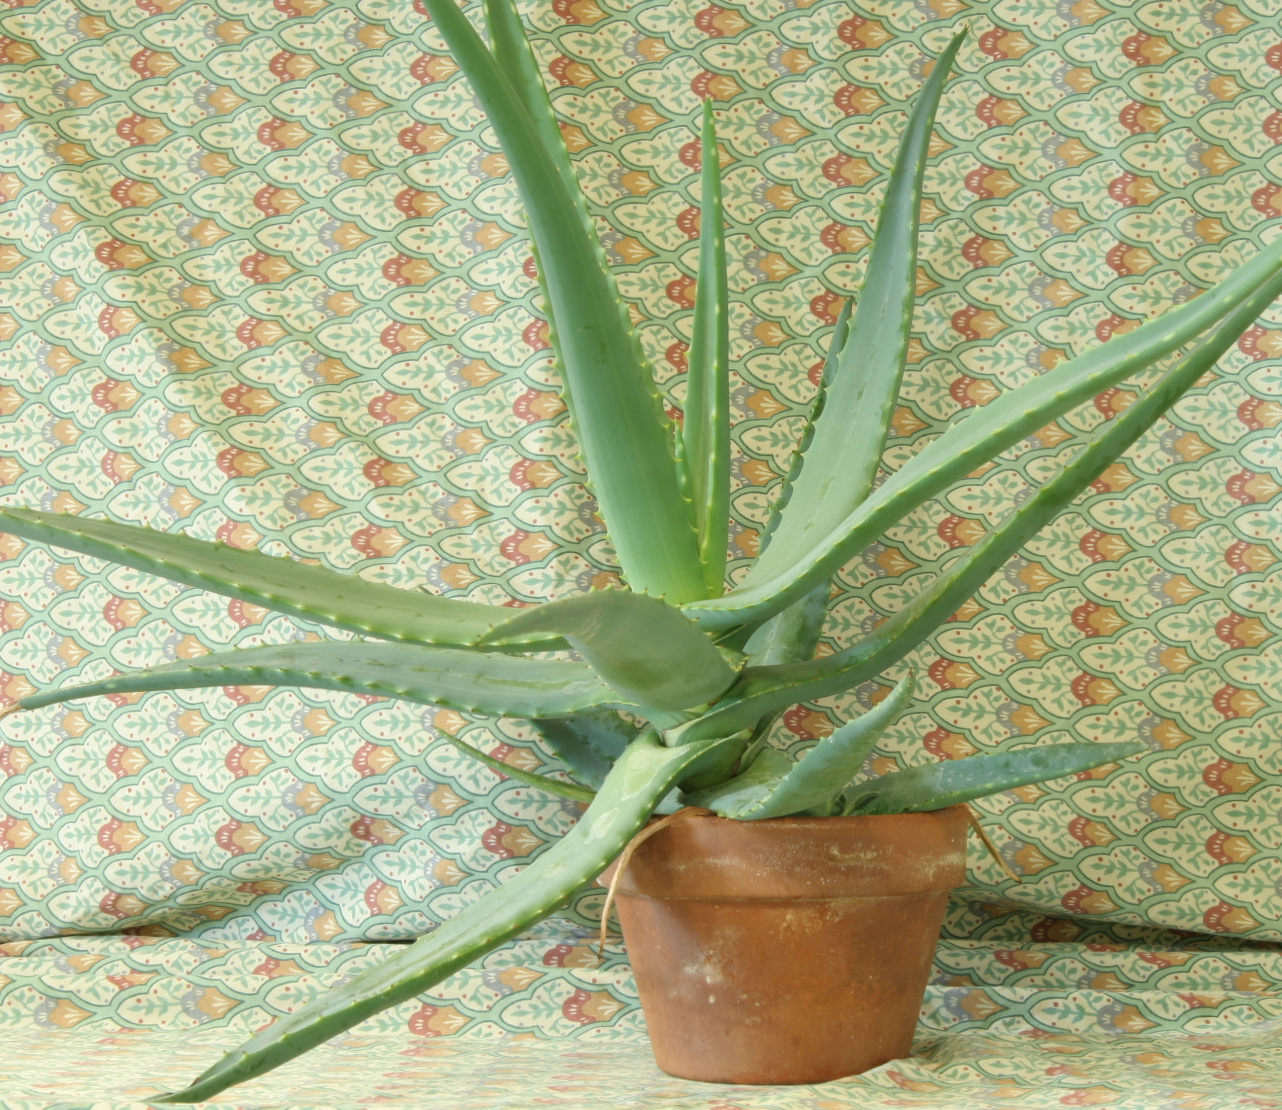
\includegraphics[width=\linewidth]{figs/aloeR.png}
  \caption{Planta pela câmera da direita.}
  \label{fig:aloeR}
\end{minipage}\hfill
\begin{minipage}[t]{0.2\textwidth}
  \centering
  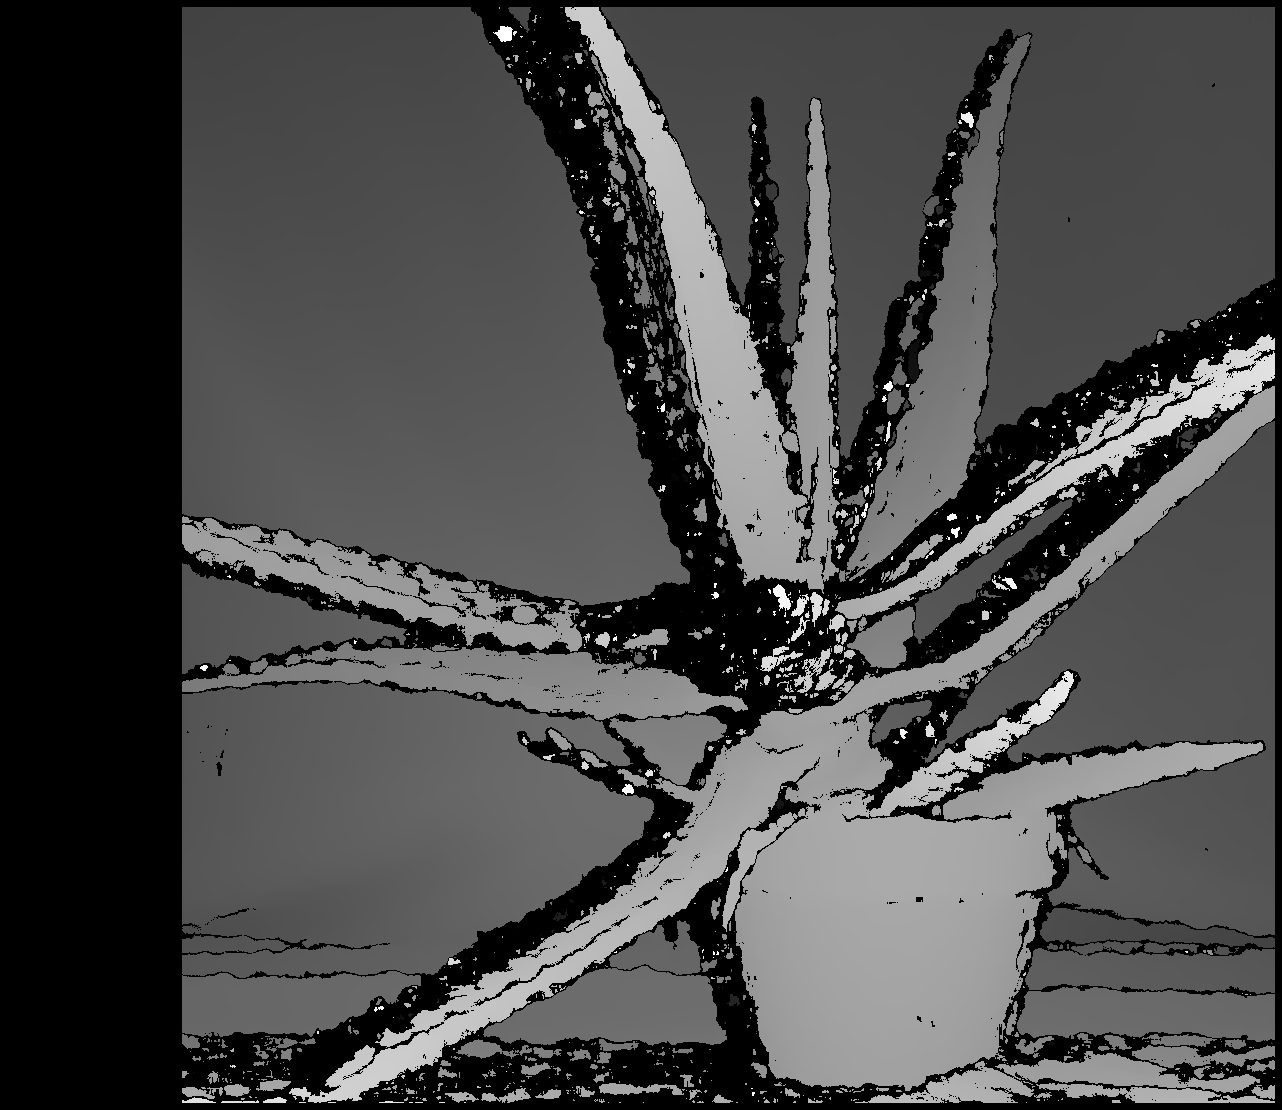
\includegraphics[width=\linewidth]{figs/aloe_disp.png}
  \caption{Mapa de disparidade.}
  \label{fig:aloe_disp}
\end{minipage}\hfill
\begin{minipage}[t]{0.2\textwidth}
  \centering
  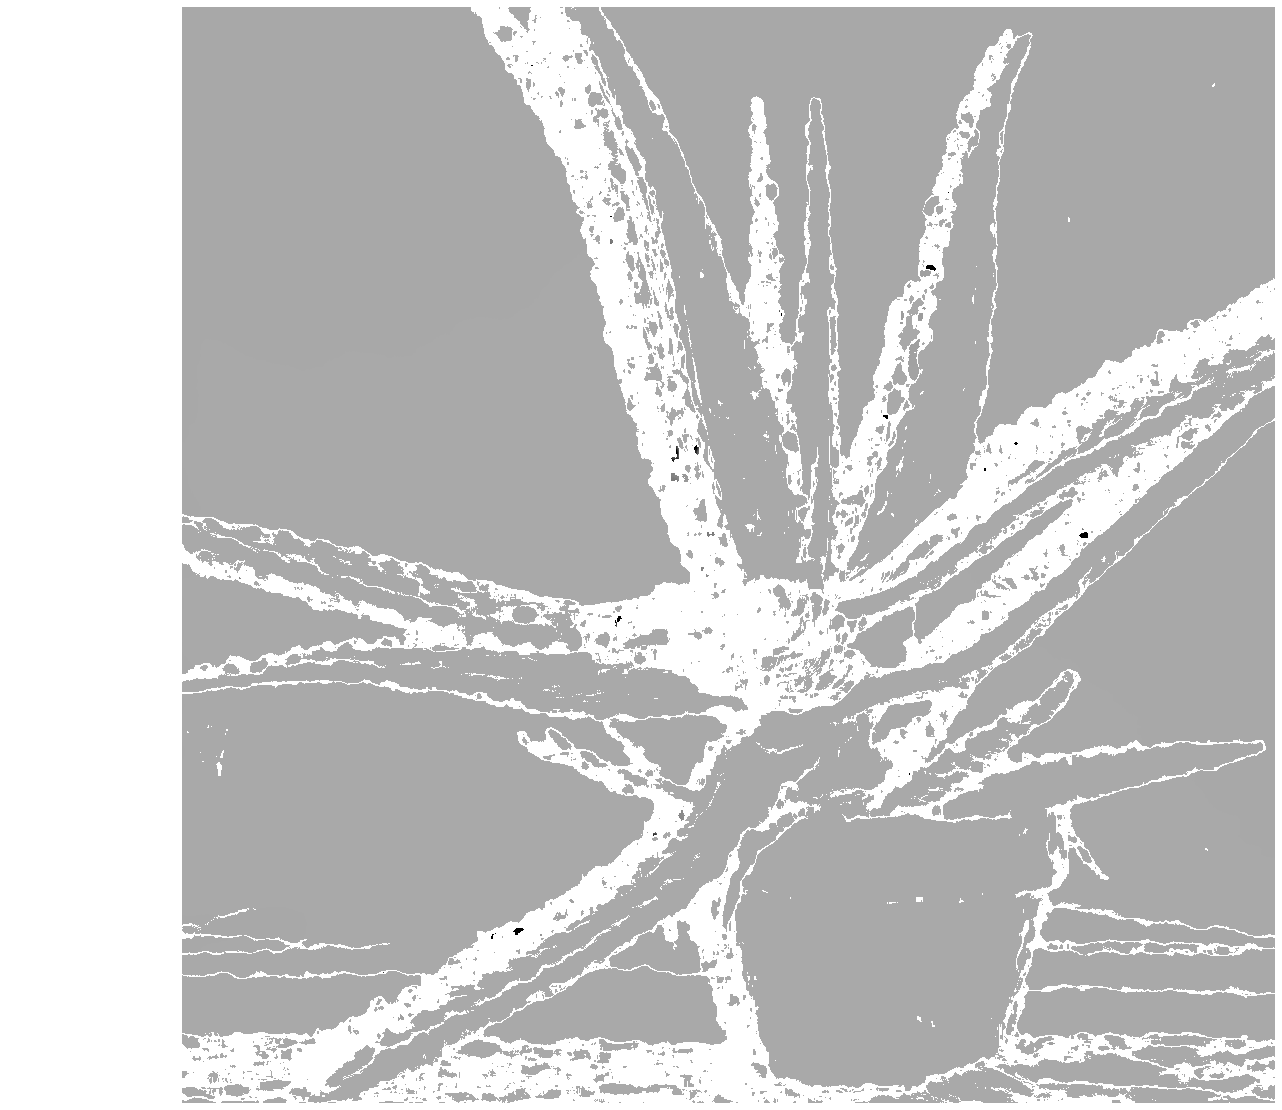
\includegraphics[width=\linewidth]{figs/aloe_depth.png}
  \caption{Mapa de profundidade.}
  \label{fig:aloe_depth}
\end{minipage}
\end{figure}

As figuras~\ref{fig:babyL} e~\ref{fig:babyR}, por outro lado, são as duas capturas da imagem de uma boneca. As figuras~\ref{fig:baby_disp} e~\ref{fig:baby_depth} são, respectivamente, o mapa de disparidade e profundidade da cena, obtidos com uma janela de tamanho 23 e um número máximo de disparidade igual a 144.

\begin{figure}[htb]
\centering
\begin{minipage}[t]{0.2\textwidth}
  \centering
  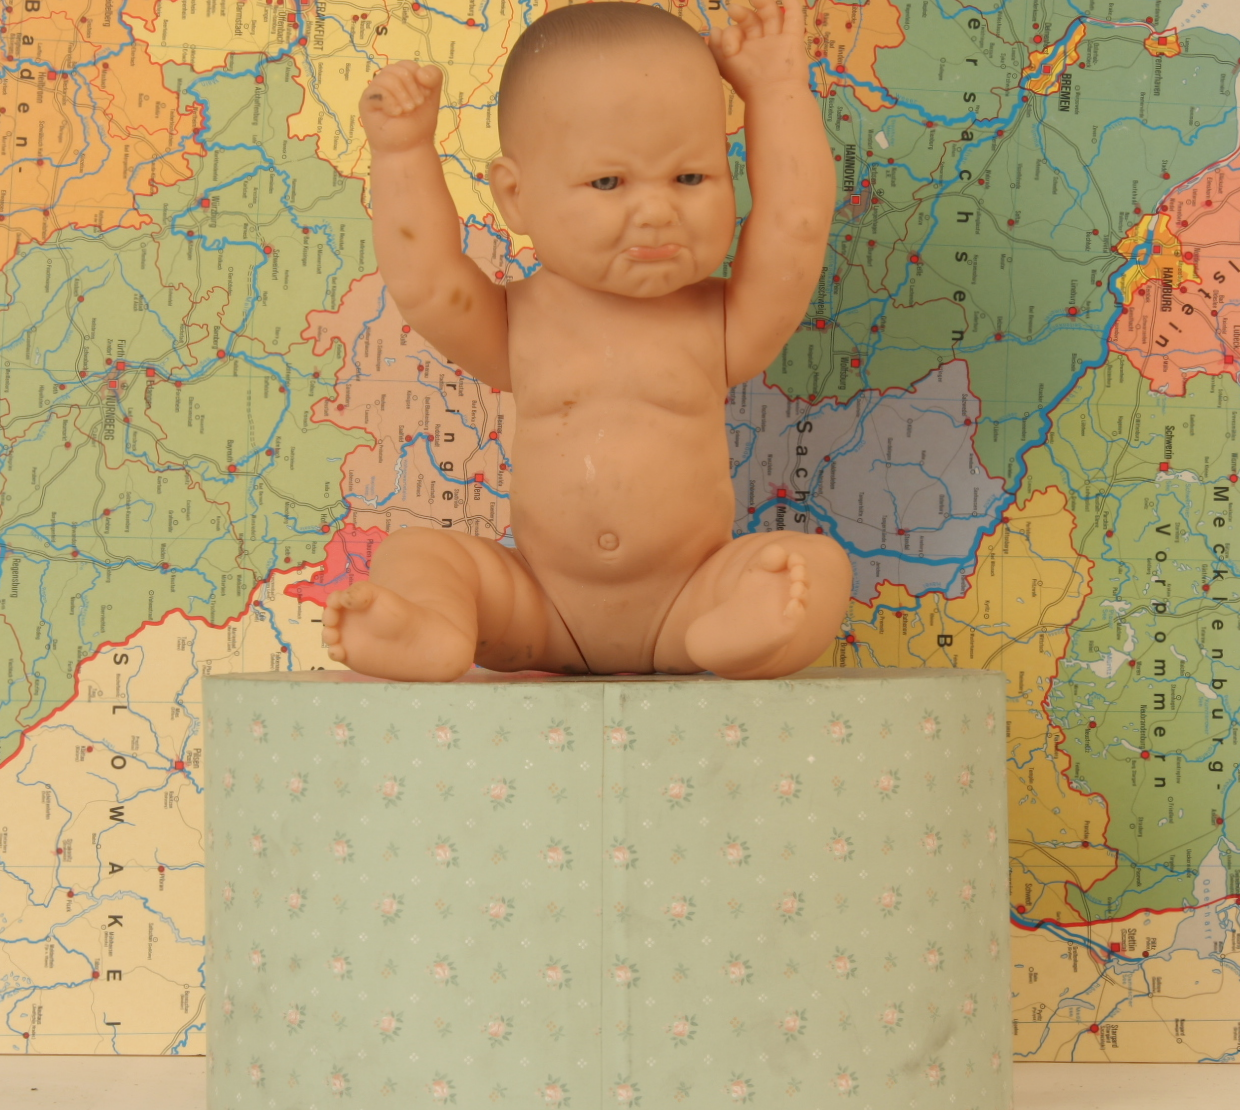
\includegraphics[width=\linewidth]{figs/babyL.png}
  \caption{Bebê pela câmera da esquerda.}
  \label{fig:babyL}
\end{minipage}\hfill
\begin{minipage}[t]{0.2\textwidth}
  \centering
  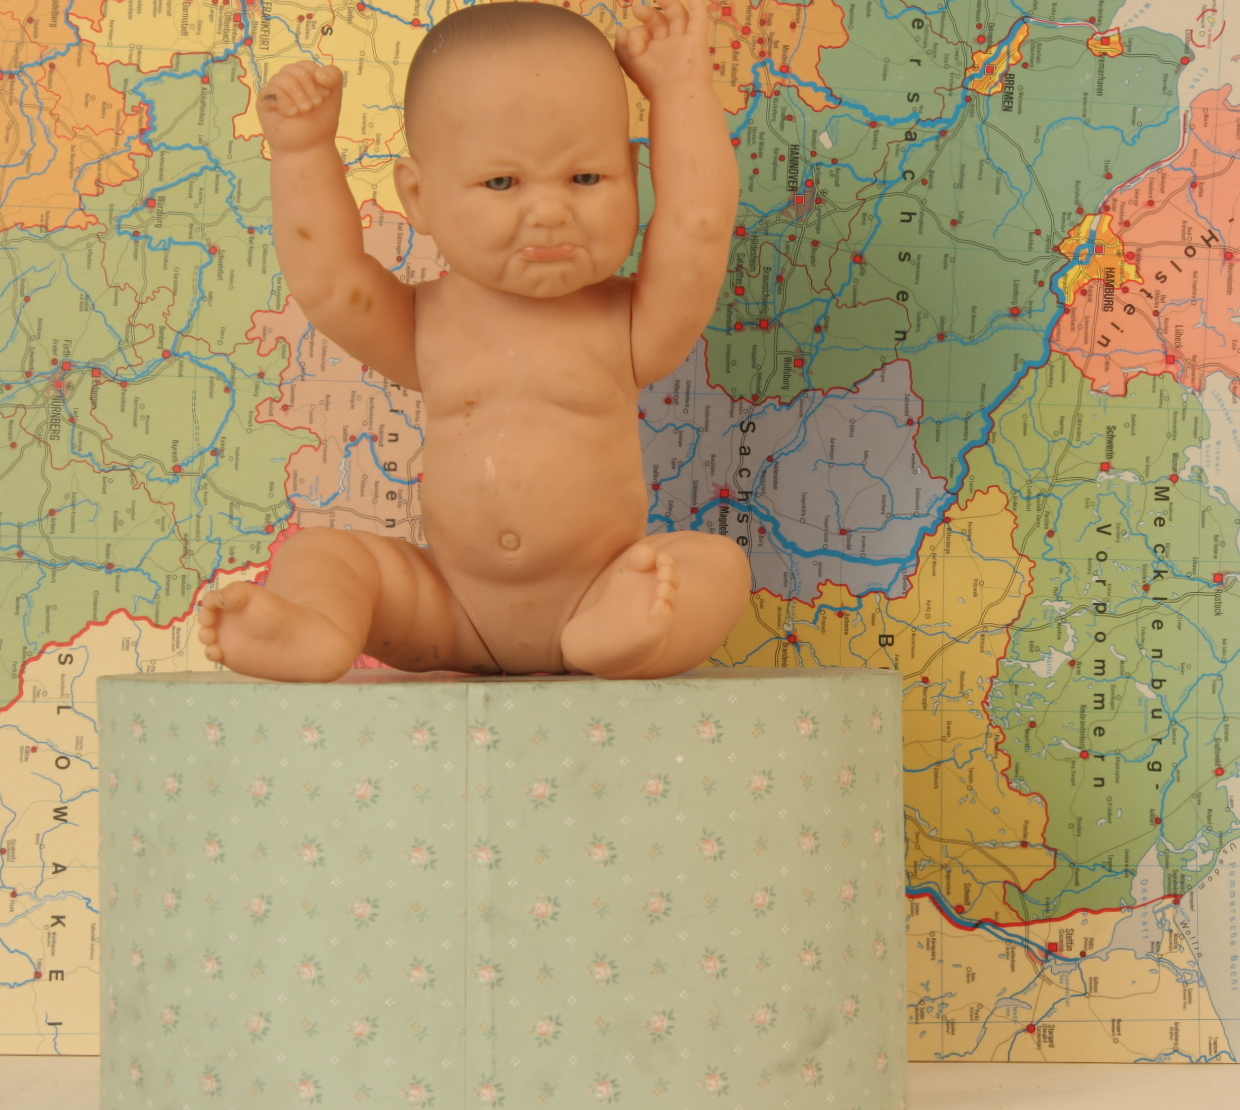
\includegraphics[width=\linewidth]{figs/babyR.png}
  \caption{Bebê pela câmera da direita.}
  \label{fig:babyR}
\end{minipage}\hfill
\begin{minipage}[t]{0.2\textwidth}
  \centering
  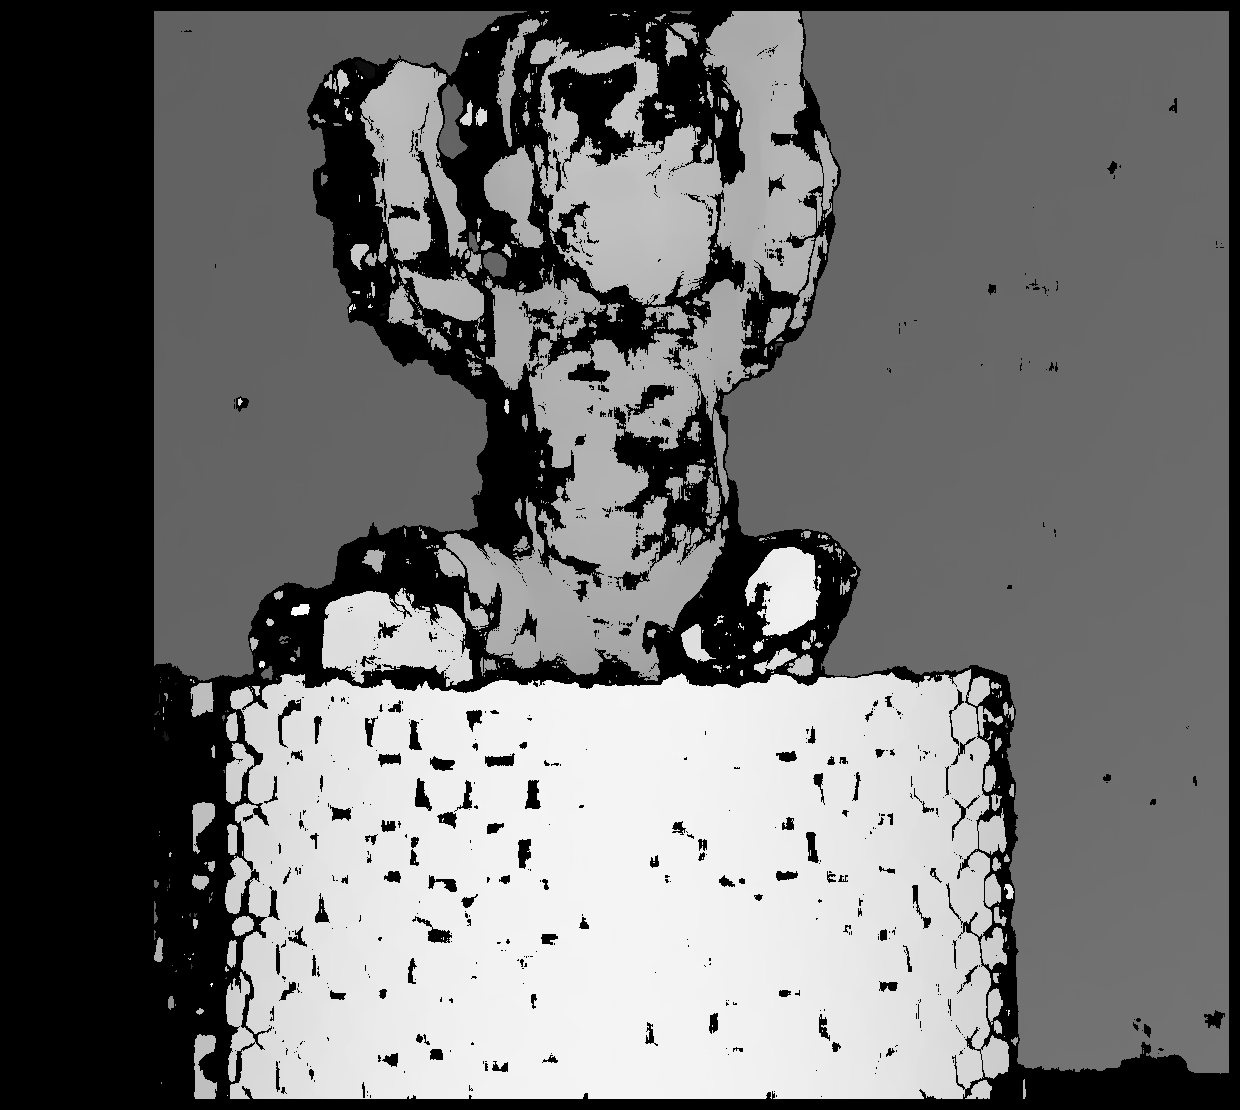
\includegraphics[width=\linewidth]{figs/baby_disp.png}
  \caption{Mapa de disparidade.}
  \label{fig:baby_disp}
\end{minipage}\hfill
\begin{minipage}[t]{0.2\textwidth}
  \centering
  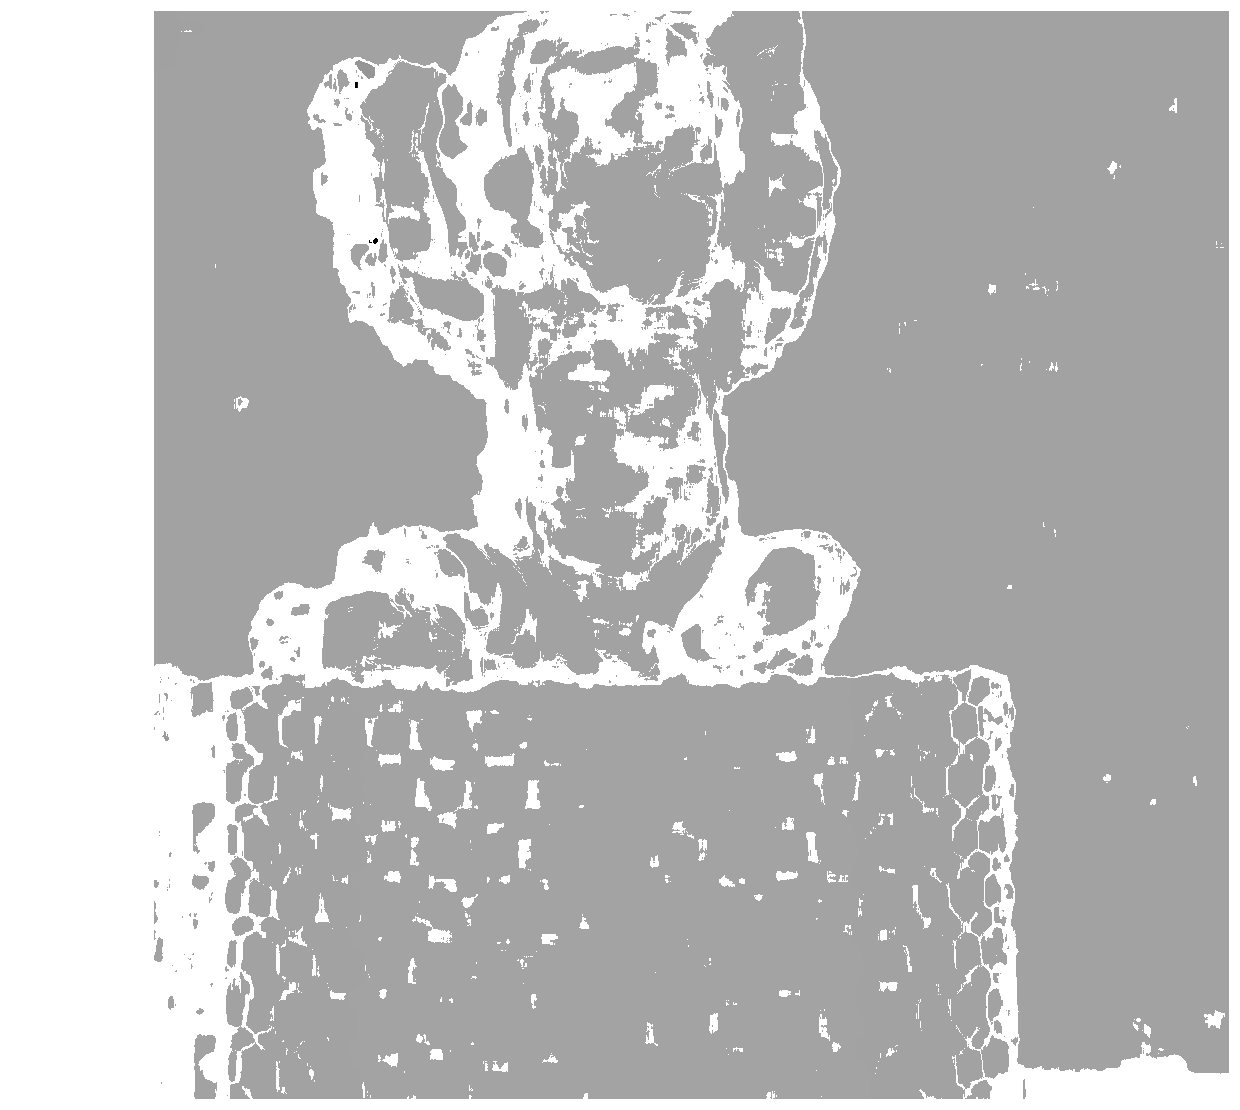
\includegraphics[width=\linewidth]{figs/baby_depth.png}
  \caption{Mapa de profundidade.}
  \label{fig:baby_depth}
\end{minipage}
\end{figure}

\subsection{Requisito 2}
A figura~\ref{fig:rec} mostra as imagens de Morpheus após retificação. Já as figuras~\ref{fig:morpheus_disp} e~\ref{fig:morpheus_depth} mostram o mapa de disparidade e profundidade obtidos por uma janela de tamanho 15 e com número máximo de disparidade igual a 256.

\begin{figure}[htb] 
\centering
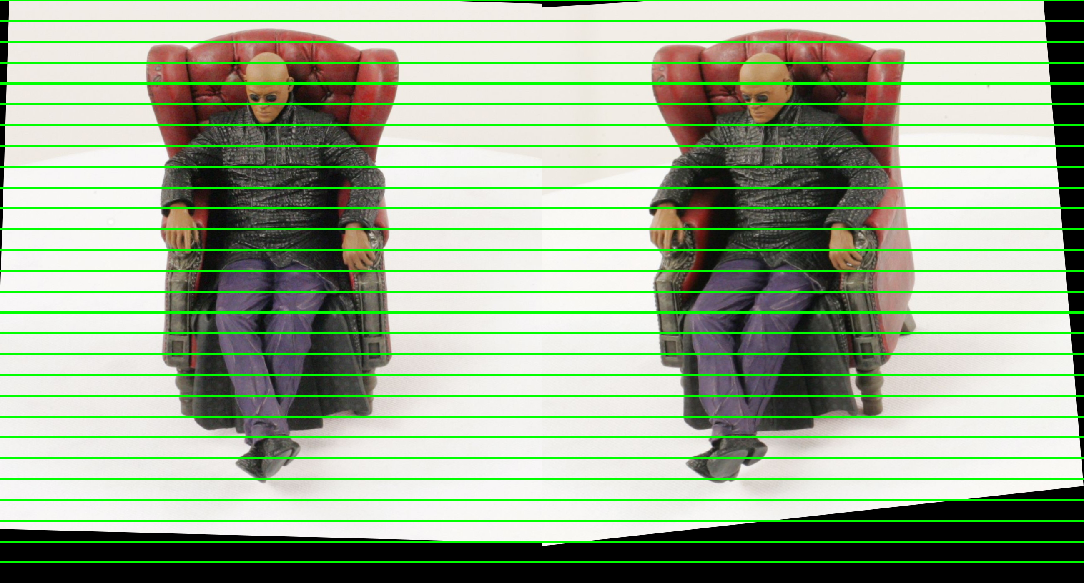
\includegraphics[width=0.6\textwidth]{figs/rec.png}
\caption{Imagens de Morpheus após retificação. As linhas horizontais indicam que os pontos correspondentes possuem o mesmo valor da coordenada $y$.\label{fig:rec}}
\end{figure}

\begin{figure}[htb]
\centering
\begin{minipage}[t]{0.3\textwidth}
  \centering
  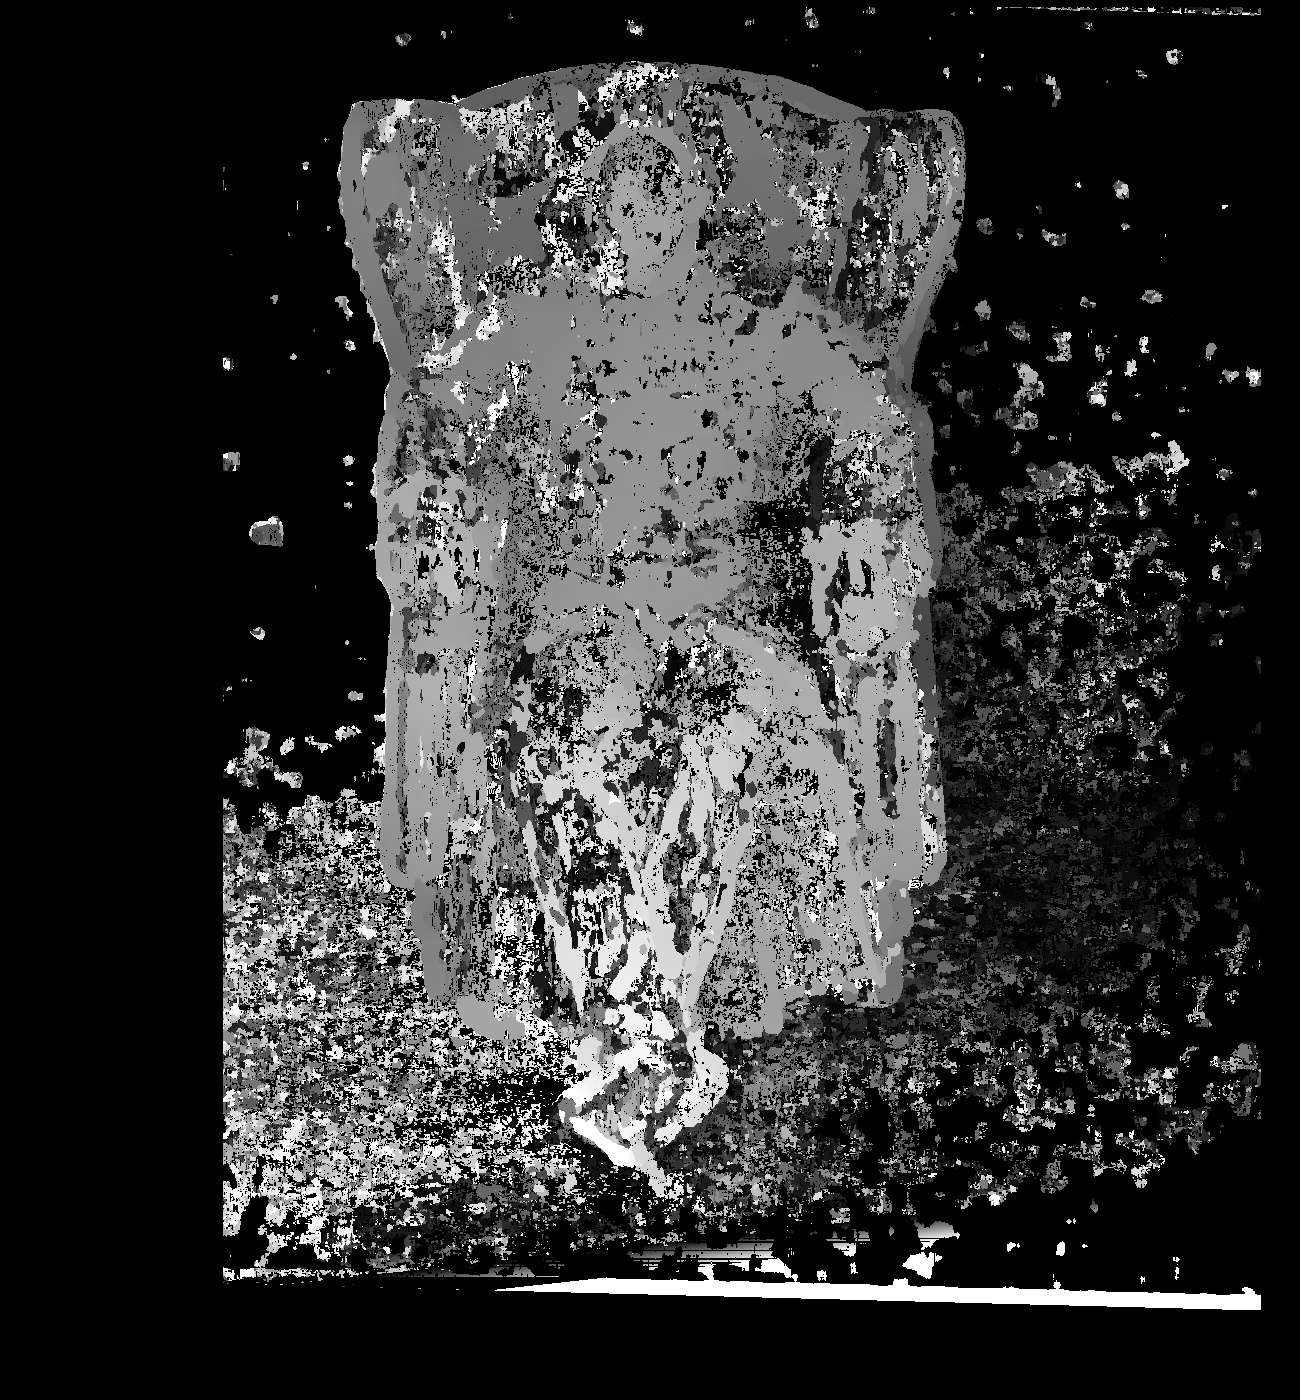
\includegraphics[width=\linewidth]{figs/morpheus_disp.jpg}
  \caption{Mapa de disparidade.}
  \label{fig:morpheus_disp}
\end{minipage}
\begin{minipage}[t]{0.3\textwidth}
  \centering
  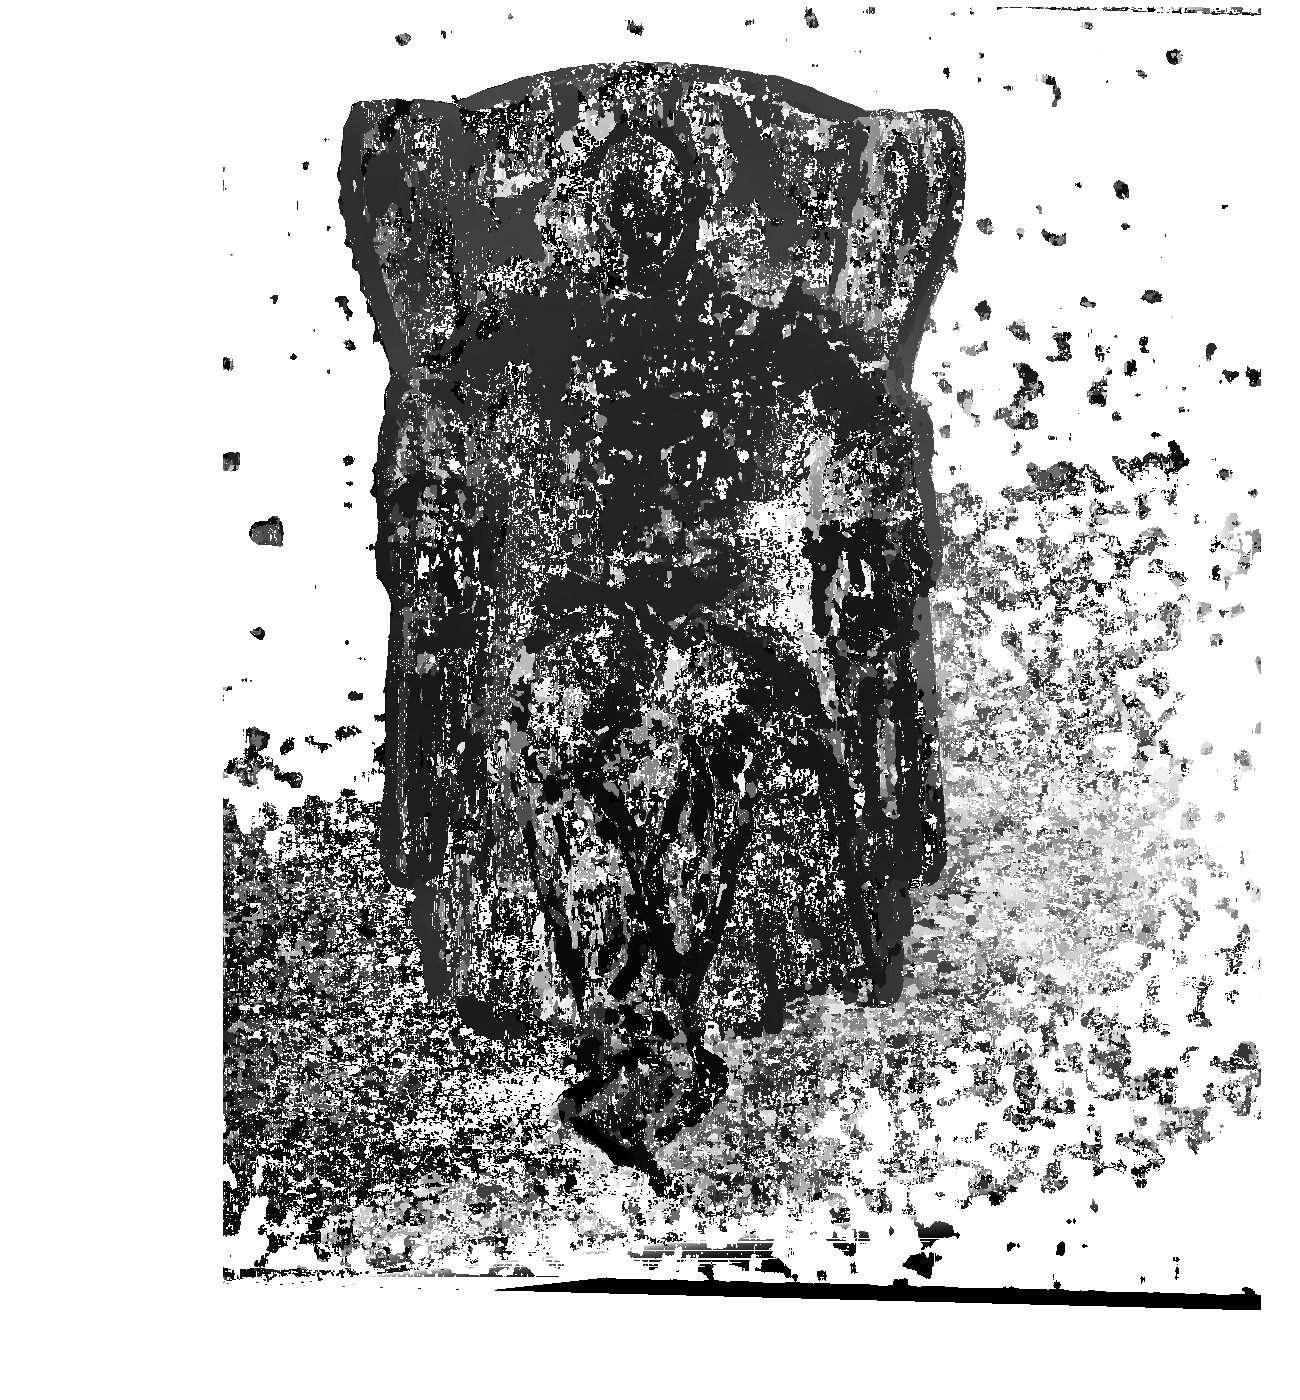
\includegraphics[width=\linewidth]{figs/morpheus_depth.jpg}
  \caption{Mapa de profundidade.}
  \label{fig:morpheus_depth}
\end{minipage}\hfill
\end{figure}

\subsection{Requisito 3}
As figuras~\ref{fig:height},~\ref{fig:width} e~\ref{fig:depth} mostram, respectivamente, onde medimos a altura, largura e profundidade da poltrona. A tabela~\ref{table:measures} exibe os valores obtidos, sendo que o erro foi obtido pelo desvio padrão de cada medida.

\begin{figure}[htb]
\centering
\begin{minipage}[t]{0.25\textwidth}
  \centering
  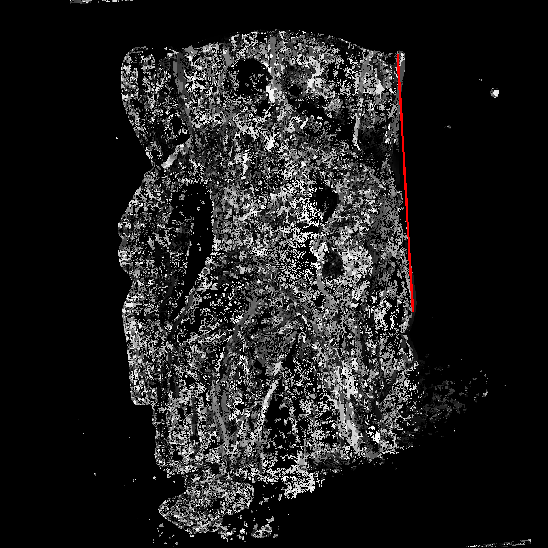
\includegraphics[width=\linewidth]{figs/height.png}
  \caption{Medida da altura.}
  \label{fig:height}
\end{minipage}\hfill
\begin{minipage}[t]{0.25\textwidth}
  \centering
  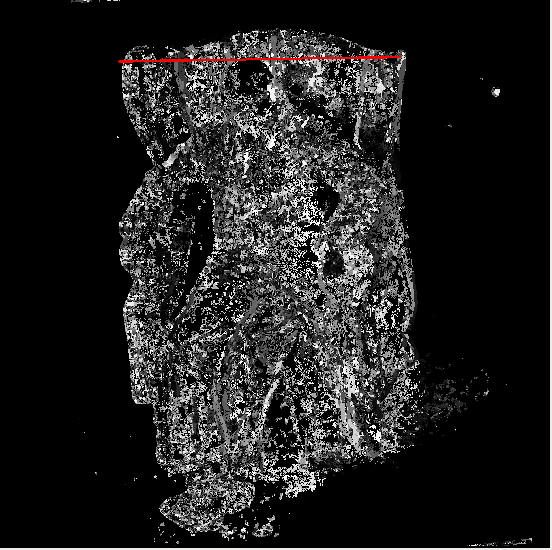
\includegraphics[width=\linewidth]{figs/width.png}
  \caption{Medida de largura}
  \label{fig:width}
\end{minipage}\hfill
\begin{minipage}[t]{0.25\textwidth}
  \centering
  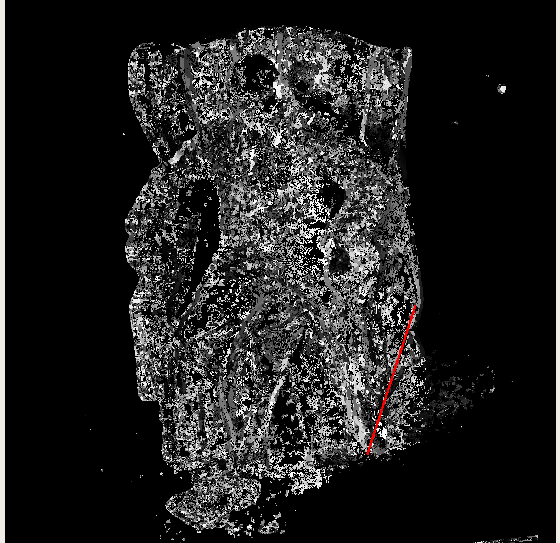
\includegraphics[width=\linewidth]{figs/depth.png}
  \caption{Medida de profundidade.}
  \label{fig:depth}
\end{minipage}
\end{figure}

\begin{table}[htb]
 \footnotesize
\caption{Medidas da poltrona.}
\label{table:measures}
\centering
\begin{tabular}{| c | c | c |}
\hline
 Altura(mm) & Largura(mm) & Profundidade(mm)\\
\hline
$184 \pm 2$ & $198 \pm 3$ & $106 \pm 4$\\
\hline

\hline
\end{tabular}
\end{table}

\section{Discussão e Conclusões}
Em relação às reconstruções das cenas da planta e da boneca, é possível constatar que a técnica trouxe bons resultados, sendo possível identificar a forma da planta e da boneca sobre a caixa, com um certo grau de detalhamento. Destacamos que o mapa de profundidade é praticamente um negativo do mapa de disparidade, o que vai ao encontro do esperado teoricamente, uma vez que a profundidade é inversamente proporcional à disparidade.

Quanto à reconstrução da cena que envolve um boneco do personagem Morpheus, inicialmente notamos que a retificação foi satisfatória, já que os pontos correspondentes se encontram dentro da mesma linha horizontal. Os mapas de profundidade e disparidade, igualmente, são razoáveis, sendo que o boneco sobre a poltrona se apresentam mais próximos que o fundo e os contornos são perceptíveis, inclusive em relação à pose de Morpheus.

Tanto no caso do requisito 1, quanto no do requisito 2, percebemos que quanto maior o tamanho da janela de busca de pixeis correspondentes, maior a suavização do mapa de disparidade. Como o valor ideal de tal parâmetro variava para cada imagem, optamos por deixar o usuário escolhê-lo em tempo real.

Os valores encontrados para as dimensões de uma caixa capaz de guardar a poltrona também são razoáveis. Todos estão na ordem dos milímetros, o que parece ser compatível com o tamanho de um boneco, embora não tenhamos os valores verdadeiros deste. Por outro lado, no momento do cálculo das medidas era comum a presença de claros \textit{outliers}, com medidas na ordem dos metros. Isso pode ocorrer por decorrência de um clique do mouse em um região onde não foi possível calcular a disparidade, que no momento de conversão para profundidade acaba assumindo um valor muito grande.

O principal problema evidenciado pelos resultados é a dificuldade do algoritmo em encontrar correspondência de pontos em regiões uniformes, como as paredes presentes nas imagens das plantas e do bebê e o fundo das imagens do Morpheus. No primeiro caso, tal dificuldade acarreta a má identificação da profundidade da parede: os pontos da parede deveriam ser os pontos com maior profundidade, mas não são identificados assim. No caso do Morpheus, os pontos do fundo sequer tem sua disparidade identificada.

Uma possível solução para isso seria o uso combinado com outras técnicas para a estimativa de profundidade de regiões homogêneas, como a segmentação, por exemplo, e o uso de informações de cores.



\clearpage
\bibliography{refs}
\end{document}
